\documentclass[11pt]{exam}
\usepackage[margin=0.7in]{geometry}
\usepackage{amsmath,amssymb}
\usepackage{colortbl}
\usepackage{multicol}
\usepackage{tikz,pgfplots}
\usepackage{soul}
\usepackage{circledsteps}

\newcommand{\blank}[1]{\underline{\hspace*{#1}}}
\newcommand{\ds}{\displaystyle}
\newcommand{\mymod}{~\mathrm{mod}~}


\begin{document}
\pagestyle{empty}
\graphicspath{{/home/brian/Dropbox/HSC/Spring16/Math111/}}

\subsection*{Midterm 2 Review \hfill Math \& Society}

\textit{The following problems are similar to ones you might see on the midterm exam. There is a also a list of terms \& facts you should memorize on the last page.}

\begin{questions}

\question A school district has 3 different elementary schools.  The enrollment (number of students) for each of the 3 schools is shown below. The school district wants to apportion its elementary school teachers to the schools proportional to the number of students.
\begin{center}
\begin{tabular}{l|ccc|c}
School & A & B & C & Total \\ \hline
Enrollment & 69 & 570 & 641 & 1280 
\end{tabular}
\end{center}

\begin{parts}
\part If the district has 120 elementary school teachers, what is the standard divisor? What are its units?
\begin{solution}
The standard divisor is 10.67 students per teacher.
\end{solution}
\vfill

\part What is the standard quota for each school? 
\begin{solution}
The standard quotas are $A: 6.46875$, $B: 53.4375$, and $C: 60.0938$. 
\end{solution}
\vfill

\part If the district uses Hamilton's method to apportion the teachers, how many teachers will each school get?
\begin{solution}
A gets 7, B gets 53 and C gets 60. 
\end{solution}
\vfill

\part What if the district hires one more teacher, increasing the number of elementary school teachers to 121.  What would Hamilton's method apportionment be in that case?  
\begin{solution}
A gets 6, B gets 54 and C gets 61. 
\end{solution}
\vfill

\part Which of the following apportionment problem best describes the situation above?
\begin{choices}
\CorrectChoice Alabama paradox
\choice New states paradox
\choice Population paradox
\choice Lower quota violation
\choice Upper quota violation
\end{choices}
\bigskip

\part If the district used Jefferson's method to apportion the teachers, how should it adjust the standard divisor to get a divisor that apportions the teachers correctly? 
\begin{choices}
\choice Increase the divisor.
\CorrectChoice Decrease the divisor.
\choice Don't change the divisor.
\choice There is not enough information to know which way to adjust the divisor.
\end{choices}

\end{parts}

\newpage
\question Consider the graph below. 
\begin{center}
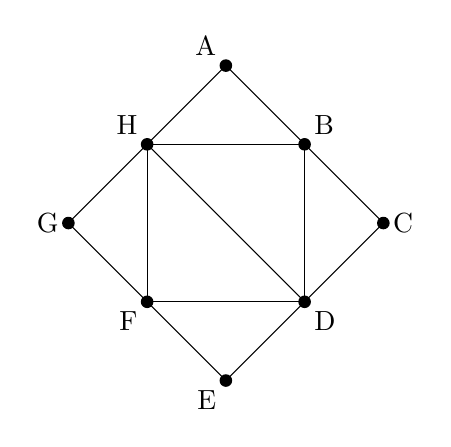
\begin{tikzpicture}
\draw (0,2) -- (2,0) -- (0,-2) -- (-2,0) -- cycle;
\draw (1,1) -- (1,-1) -- (-1,-1) -- (-1,1) -- cycle;
\draw (-1,1) -- (1,-1);
\fill (0,2) circle (0.08) node[above left] {A};
\fill (2,0) circle (0.08) node[right] {C};
\fill (0,-2) circle (0.08) node[below left] {E};
\fill (-2,0) circle (0.08) node[left] {G};
\fill (1,1) circle (0.08) node[above right] {B};
\fill (1,-1) circle (0.08) node[below right] {D};
\fill (-1,-1) circle (0.08) node[below left] {F};
\fill (-1,1) circle (0.08) node[above left] {H};
\end{tikzpicture}
\end{center}

\begin{parts}
\part Does the graph have an Euler circuit?  Why or why not?
\begin{solution}
No, not all of the vertices have even degrees.
\end{solution}
\vfill

\part Does the graph have an Euler path?  Why or why not?  
\begin{solution}
Yes, there are exactly two odd degree vertices (H and D). 
\end{solution}
\vfill

\part What is the sum of the degrees of the vertices in this graph?
\begin{solution}
A, C, E, and G have degree 2.  B and F have degree 4, and H, D both have degree 5, so the total is 26.  
\end{solution}
\vfill

\end{parts}

\question Draw a tree that has a degree 4 vertex, a degree 3 vertex, and a degree 2 vertex. 
\begin{solution}
There are many possible answers, but here is one:
\begin{center}
\begin{tikzpicture}
\draw (0,0) -- (1,0) -- (2,0) -- (3,0) -- (4,0);
\draw (1,-1) -- (1,1);
\draw (2,-1) -- (2,0);
\fill (0,0) circle (0.08);
\fill (1,0) circle (0.08);
\fill (1,-1) circle (0.08);
\fill (1,1) circle (0.08);
\fill (2,0) circle (0.08);
\fill (2,-1) circle (0.08);
\fill (3,0) circle (0.08);
\fill (4,0) circle (0.08);
\end{tikzpicture}
\end{center}
\end{solution}
\vfill

\newpage

\question Use the mileage chart below to find the minimum spanning tree connecting these five cities.  
\begin{center}
\begin{tabular}{l|ccccc}
& Boston & Buffalo & Chicago & Columbus & Louisville \\ \hline
Boston & -- & 446 & 963 & 735 & 941 \\ 
Buffalo & 446 & -- & 522 & 326 & 532 \\ 
Chicago & 963 & 522 & -- & 308 & 292 \\
Columbus & 735 & 326 & 308 & -- & 209 \\
Louisville & 941 & 532 & 292 & 209 & -- 
\end{tabular}
\end{center}
\begin{solution}
Start with Columbus to Louisville (209).  Then add Chicago to Louisville (292).  You can't add Chicago to Columbus (308), so the next cheapest route is Buffalo to Columbus (326).  Then add Buffalo to Boston (446).  Now all five cities are connected, so you are done.  
\end{solution}
\vfill

\question Which of the following graphs must be a tree?  Circle all that are.  
\begin{choices}
\CorrectChoice An ancestry graph.  People are vertices; edges connect parents to their children.
\choice Friends network.  People are vertices; edges connect people who are friends.  
\choice Railway network. Cities are vertices; railway routes are the edges.
\end{choices}
\bigskip

\question If a graph has 100 vertices, and every vertex is degree 3, then how many edges does the graph have?
\begin{solution}
Since the sum of the degrees of the vertices is twice the number of edges, there must be 150 edges. 
\end{solution}
\vfill

\question Some people argue that the United States should switch back to Hamilton's method to apportion the seats in Congress.  Which of the following is \emph{not} an advantage of Hamilton's method. 
\begin{choices}
\CorrectChoice There are no paradoxes. 
\choice No state ever gets more than its upper quota.
\choice No state ever gets less than its lower quota.
\end{choices}

\newpage
\question Let $v = \begin{pmatrix} 0.2 &  0.2 & 0.6 \end{pmatrix}$ and let $Q = \begin{pmatrix} 0.2 & 0.2 & 0.6 \\ 1 & 0 & 0 \\ 0 & 1 & 0 \end{pmatrix}$
\begin{parts}
\part Calculate $vQ$.  Based on your calculation, is $v$ a stationary distribution for $Q$?  
\begin{solution}
$$ vQ = \begin{pmatrix}  0.24 & 0.64 & 0.12 \end{pmatrix}.$$ 
Since  $vQ$ is not the same as $v$, it is not a stationary distribution.  
\end{solution}

\vfill

\part The matrix $Q= \begin{pmatrix} 0.2 & 0.2 & 0.6 \\ 1 & 0 & 0 \\ 0 & 1 & 0 \end{pmatrix}$ is a transition matrix for a Markov chain.  Draw and label the graph for that Markov chain. 
\begin{solution}
\begin{center}
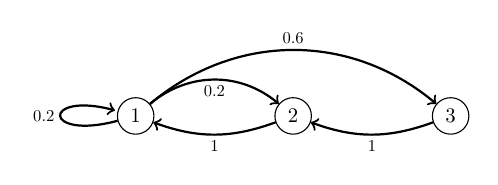
\begin{tikzpicture}
\path (0,0) node[draw,shape=circle,scale=0.75] (A) {1};
\path (2,0) node[draw,shape=circle,scale=0.75] (B) {2};
\path (4,0) node[draw,shape=circle,scale=0.75] (C) {3};

\path[thick,->]  (A) edge [bend left=40] node[below, scale=0.6] {$0.2$} (B);
\path[thick,->]  (A) edge [bend left=40] node[above, scale=0.6] {$0.6$} (C);
\path[thick,->]  (A) edge [loop left, scale=2] node[left,scale=0.6] {$0.2$} (A);
\path[thick, ->] (B) edge  [bend left=20]  node[below, scale=0.6] {$1$} (A);
\path[thick, ->] (C) edge  [bend left=20]  node[below, scale=0.6] {$1$} (B);

\end{tikzpicture}
\end{center}
\end{solution}
\vfill

\end{parts}

\question Consider the Markov chain shown below. 
\begin{center}
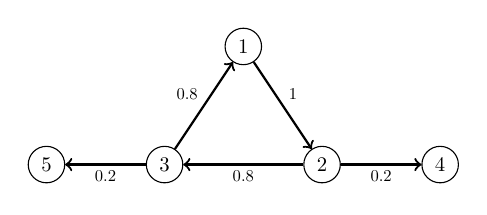
\begin{tikzpicture}
\path (0,1) node[draw,shape=circle,scale=0.75] (A) {1};
\path (1,-0.5) node[draw,shape=circle,scale=0.75] (B) {2};
\path (-1,-0.5) node[draw,shape=circle,scale=0.75] (C) {3};
\path (2.5,-0.5) node[draw,shape=circle,scale=0.75] (D) {4};
\path (-2.5,-0.5) node[draw,shape=circle,scale=0.75] (E) {5};

\path[thick,->] (A) edge  node[above right,scale=0.6] {$1$} (B);
\path[thick,->] (B) edge  node[below,scale=0.6] {$0.8$} (C);
\path[thick,->] (C) edge  node[above left,scale=0.6] {$0.8$} (A);
\path[thick,->] (B) edge  node[below,scale=0.6] {$0.2$} (D);
\path[thick,->] (C) edge  node[below,scale=0.6] {$0.2$} (E);
\end{tikzpicture}
\end{center}
\begin{parts}
\part What are the strongly connected components of this Markov chain?  Which components are final? 
\begin{solution}
There are 3 strongly connected components. They are $\{1,2,3\}$, $\{4\}$, and $\{5\}$.  The last two are final.  
\end{solution}
\vfill

\part The transition matrix for this Markov chain is $Q = \begin{pmatrix} 0 & 1 & 0 & 0 & 0 \\ 0 & 0 & 0.8 & 0.2 & 0 \\ 0.8 & 0 & 0 & 0 & 0.2 \\ 0 & 0 & 0 & 1 & 0 \\ 0 & 0 & 0 & 0 & 1 \end{pmatrix}$.  If you raise this matrix to a large power $k$ (anything greater than 100), you will get 
$$Q^k = \begin{pmatrix} 0 & 0 & 0 & 0.555 & 0.444 \\  0 & 0 & 0 & 0.555 & 0.444 \\  0 & 0 & 0 & 0.444 & 0.555 \\ 0 & 0 & 0 & 1 & 0 \\ 0 & 0 & 0 & 0 & 1 \end{pmatrix}.$$
If you start in state 3, what is the probability that you will eventually end up in state 4?  


\begin{solution}
The probability is the number in row 3, column 4 : 0.444.  
\end{solution}
\vfill
\end{parts}

\newpage

\question About 40\% of American adults are obese. About 10\% of American adults have type II diabetes. And about 9\% of American adults are both obese and have type II diabetes. Let A be the event that a randomly selected American adult is obese, and let B be the event that they have type II diabetes. 
\begin{parts}
\part Are A and B independent?  Explain how you can tell. 
\begin{solution}
A and B are not independent because $P(A \text{ and } B) = 9\%$ which is not $P(A) \cdot P(B) = (0.10)(0.40) = 4\%$.  
\end{solution}
\vfill

\part Find $P(\text{not } A)$.
\begin{solution}
$$P(\text{not } A) = 100\% - 40\% = 60\%.$$ 
\end{solution}
\vfill


\part Find $P(A \text{ or } B)$.
\begin{solution}
$$P(A \text{ or } B) = 40\% + 10\% - 9\% = 41 \%.$$
\end{solution}
\vfill

\part Find $P(A \, | \, B)$. 
\begin{solution}
$$P(A | B) = \frac{P(A \text{ and } B)}{P(B)} = 9/10 = 90\%.$$
\end{solution}
\vfill

\end{parts}

\end{questions}

\newpage

\section*{Midterm 2 Study Guide}

Midterm 2 will focus on the following topics.  Make sure you know all of the terms listed in bold.  

\begin{description}
\item[Apportionment] Know how each of the following apportionment methods work: \textbf{Hamilton's}, \textbf{Jefferson's}, \textbf{Adam's}, and \textbf{Webster's methods}. Be able to identify the \textbf{standard divisor} and \textbf{standard quotas}.  Know the advantages and disadvantages of the different methods:

\begin{itemize}
\item Hamilton's method has no \textbf{quota violations}, but it can have the \textbf{Alabama paradox}, the \textbf{new states paradox}, and the \textbf{population paradox}. 

\item The divisor methods (Adams, Jeffersons, and Websters) don't have paradoxes, but they can all have quota violations.  Jefferson's method is biased in favor of big states, so they sometimes get too many seats (\textbf{upper quota violations}), Adam's method is biased against big states (so they can have \textbf{lower quota violations}).  Webster's method (and also the Huntington-Hill method that Congress currently uses) is not biased, but it can have both upper and lower quota violations.  
\end{itemize}

\item[Graph Theory] Know what the \textbf{degree} of a vertex is.  Know that the sum of the degrees of all the vertices in a graph is twice the number of edges.  Know that a \textbf{tree} is a connected graph with no cycles.  For a tree you should know that $V = E+1$ and what that means.  You should know when a graph has an \textbf{Euler path} or an \textbf{Euler circuit} and what those are.  

\item[Markov chains] Be able to convert a description of a Markov chain to a graph and/or a \textbf{transition matrix}.  Know how to multiply matrices, and understand the meaning of a power of a transition matrix.  You should also know how to find the \textbf{strongly connected components} of a Markov chains and be able to recognize the \textbf{final components}.  If the powers $Q^k$ of the transition matrix $Q$ converge, then the rows of the matrix $Q^k$ when $k$ is large are each \textbf{stationary distributions} $v$ of the Markov chain which means that 
$$v Q = v.$$

\item[Probability] You should be able to determine if all of the elements of a \textbf{sample space} are \textbf{equiprobable} and how to calculate the probability of an \textbf{event} in an equiprobable model. Know the basic probability rules: \textbf{Complementary events}, \textbf{Addition rule}, and \textbf{Multiplication rule for independent events}.  Know that two events are \textbf{independent} when knowing that one has happened does not change the probability for the other. Know how to calculate a \textbf{weighted average}, and how to use weighted averages to find the \textbf{expected value} of a probability model with numerical outcomes.  Finally, you should know the \textbf{Law of Large Numbers}.   

\end{description}

\end{document}
